\documentclass[10pt]{beamer}
\usetheme[
%%% options passed to the outer theme
%    hidetitle,           % hide the (short) title in the sidebar
%    hideauthor,          % hide the (short) author in the sidebar
%    hideinstitute,       % hide the (short) institute in the bottom of the sidebar
%    shownavsym,          % show the navigation symbols
%    width=2cm,           % width of the sidebar (default is 2 cm)
%    hideothersubsections,% hide all subsections but the subsections in the current section
%    hideallsubsections,  % hide all subsections
%    right                % right of left position of sidebar (default is right)
  ]{Aalborg}

\definecolor{aaublue}{RGB}{33,26,82}
\definecolor{aaugrey}{RGB}{84,97,110}

% If you want to change the colors of the various elements in the theme, edit and uncomment the following lines
% Change the bar and sidebar colors:
\setbeamercolor{Aalborg}{fg=aaublue!10,bg=aaugrey!60}
%\setbeamercolor{sidebar}{bg=blue!74}
% Change the color of the structural elements:
\setbeamercolor{structure}{fg=aaublue}
 \setbeamercolor{subtitle}{fg=aaugrey}
% Change the frame title text color:
\setbeamercolor{frametitle}{fg=aaublue}
% Change the normal text color background:
%\setbeamercolor{normal text}{bg=aaugrey!10}
% ... and you can of course change a lot more - see the beamer user manual.
\usebackgroundtemplate{
\includegraphics[width=\paperwidth]{img/background}}

\usepackage[utf8]{inputenc}
\usepackage[english]{babel}
\usepackage[T1]{fontenc}
% ... or whatever. Note that the encoding and the font should match. If T1
% does not look nice, try deleting the line with the fontenc.
\usepackage{lmodern} %optional

% colored hyperlinks
\newcommand{\chref}[2]{%
  \href{#1}{{\usebeamercolor[bg]{Aalborg}#2}}
}

\title[Centralized State Estimation\\ of Distributed Maritime Autonomous Surface Oceanographers]% optional, use only with long paper titles
{Centralized State Estimation of Distributed Maritime Autonomous Surface Oceanographers}

%\subtitle[v.\ 0.1.1] %optional
%{v.\ 0.1.1}

\author[12gr730]{% optionally input the group number, use only with lots of authors
  Attila Fodor \and Rasmus L. Christensen \and Frederik Juul \and Tudor Muresan \and Nick \O stergaard\\
  {{\tt \{afodor12,ralch,fjuul,tmures12,nickoe\}@es.aau.dk}}
}
% - Give the names in the same order as they appear in the paper.
% - Use the \inst{?} command only if the authors have different
%   affiliation. See the beamer manual for an example

%specify some optional logos
\pgfdeclareimage[height=1.2cm]{mainlogo}{aau_logo.pdf} % placed in the upper left/right corner
\logo{\pgfuseimage{mainlogo}}

\pgfdeclareimage[height=0.75cm]{logo2}{tu-logo} % placed in the lower left/right corner if the \pgfuseimage{logo2} command is uncommented in the \institute command below

\institute[
%  {\pgfuseimage{logo2}}\\ %insert a company or department logo
  Dept.\ of Electronic Systems,\\
  Aalborg University,\\
  Denmark
] % optional - is placed in the bottom of the sidebar on every slide
{%
  Department of Electronic Systems,\\
  Aalborg University,\\
  Denmark
  
  %there must be an empty line above this line - otherwise some unwanted space is added between the university and the country (I do not know why;( )
}
\date{\today}

\begin{document}
% the titlepage
\begin{frame}[plain] % the plain option removes the sidebar and header from the title page
  \titlepage
\end{frame}
%%%%%%%%%%%%%%%%

% TOC
\begin{frame}{Agenda}{}
\tableofcontents
\end{frame}
%%%%%%%%%%%%%%%%
\section{Introduction}
\begin{frame}{Introduction}{Purpose}
  \begin{itemize}
  	\item<1-> Little to no research are currently devoted to maritime autonomous crafts.
    \item<2-> During the 2012 Fukushima accident in Japan, no measurements of the spread of radioactivity was available in the coastal zones, thus relying only on estimates. 
    \item<3-> The coastal area around Greenland has no up-to-date baymethric maps available, and with the growing interest in Greenland (both industrially and commercially) this poses a threat to the ships going in and out of the fjords.
  \end{itemize}
\end{frame}
%%%%%%%%%%%%%%%%
\begin{frame}{Introduction}{Problem Description}
Empty frame
\end{frame}

%%%%%%%%%%%%%%%%
\section{Development}
\subsection{AAUSHIP.01}
\begin{frame}{Development}{AAUSHIP.01}
\begin{itemize}
	\item<1-> The ship is designed as a non-planing deplacement craft (eg. like freight ships).
	\item<2-> Developed using rapid prototyping techniques.
	\item<3-> Developed in Rhinoceros\texttrademark using a lofting techniques.
	\item<4-> Printed on a 3D printer.
	\item<5-> Examined and the process iterated.
	\item<6-> Vaccumformed by DD-plast in Randers and assembled in the machine shop at Aalborg University.
\end{itemize}
\end{frame}

%%%%%%%%%%%%%%%%
\begin{frame}{Development}{AAUSHIP.01 Hull}
Pictures of the ship.
\end{frame}

%%%%%%%%%%%%%%%%
\begin{frame}{Development}{AAUSHIP.01 Hull}
Pictures of the ship.
\end{frame}

%%%%%%%%%%%%%%%%
\subsection{Development}
\begin{frame}{Development}{Hardware}
\begin{itemize}
	\item Fitted with 2 x 1200W engines (totally producing around 3 HP at full thrust).
	\item Fitted with 6 x 3200mAh batteries (results in a mission time of around 5 hours).
	\item 2 counter rotating 60mm propellers.
	\item Inertial Measurement Unit.
	\item Global Positioning System.
	\item A 20mW 19.2 kbps radio link @ 470 MHz
	\item Arduino Mega with a custom made shield board mounted.
    \item Retrofitted with a hydrofoil to reduce the wake and pitch of the ship.
\end{itemize}
\end{frame}

%%%%%%%%%%%%%%%%
\begin{frame}{Development}{Protocol}
The designed protocol is given as:
\end{frame}

%%%%%%%%%%%%%%%%
\begin{frame}{Development}{Distributed Control}
As the protocol takes care of packet verification, the channel can be estimated by a bernoulli variable, with outcomes of a received package either a succes or a failure.
\begin{figure}
	\begin{center}
		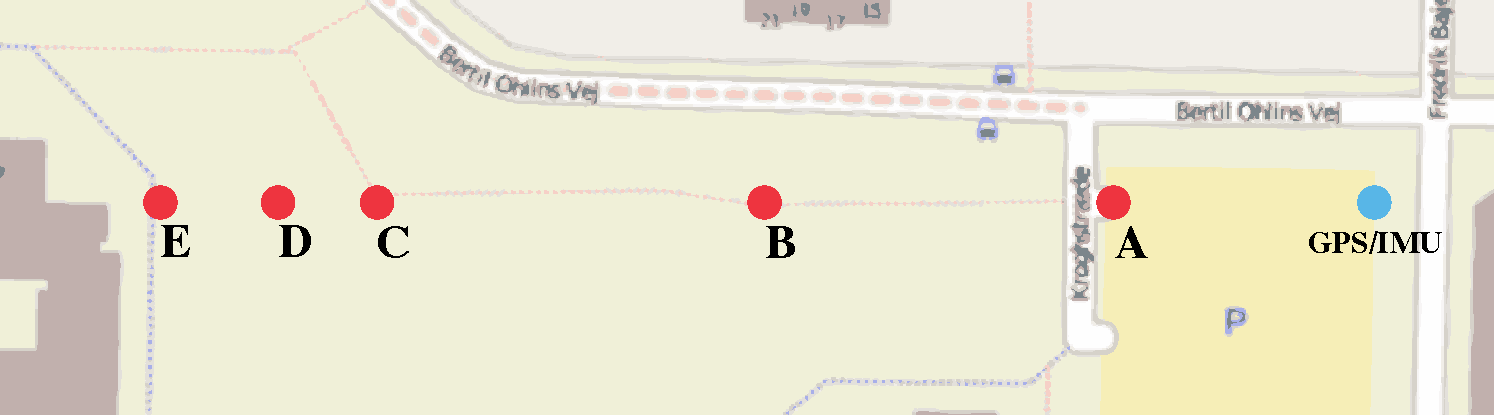
\includegraphics[width=8.2cm]{img/measpoint}
		\label{fig:measpoint}
	\end{center}
\end{figure}
The measurements make for the following distribution of the GPS with a distance of 189 metres:
\begin{align}
\lambda_\text{gps,E} = \left\{ 
  \begin{array}{l l}
    0.8643 & \quad \text{for $\lambda$ = 1}\\
    0.1357 & \quad \text{for $\lambda$ = 0}
  \end{array} \right.
\end{align}
And for the IMU also at 189 metres.
\begin{align}
\lambda_\text{imu,E} = \left\{ 
  \begin{array}{l l}
    0.8689 & \quad \text{for $\lambda$ = 1}\\
    0.1311 & \quad \text{for $\lambda$ = 0}
  \end{array} \right.
\end{align}
\end{frame}

%%%%%%%%%%%%%%%%
\begin{frame}{Development}{Kalman Filter}
The derivation of the Kalman filter is based around the position being equal to the last position, the change due to velocity and the change due to acceleration:
\begin{align}
x[n] &= x[n-1] + \dot{x}[n-1]\cdot ts + \ddot{x}[n-1]\cdot \frac{ts^2}{2}\\
\dot{x}[n] &= \dot{x}[n-1] + \ddot{x}[n-1] \cdot ts\\
\ddot{x}[n] &= -\beta \cdot \dot{x}[n-1] + \ddot{x}[n]
\end{align}
Which can be put on matrix form:
\begin{align}
\begin{bmatrix}
x[n]\\
\dot{x}[n]\\
\ddot{x}[n]
\end{bmatrix} = \begin{bmatrix}
1 & ts & \frac{ts^2}{2}\\
0 & 1 & ts\\
0 & -\beta & 0
\end{bmatrix}\begin{bmatrix}
x[n-1]\\
\dot{x}[n-1]\\
\ddot{x}[n-1]
\end{bmatrix}
\end{align}
This goes for the $y$-axis and the rotation about the $z$-axis as well.
\end{frame}

%%%%%%%%%%%%%%%%
\section{Modeling}
\subsection{Engine model}
\begin{frame}{Modeling}{Thrust/Torque Model}
The thrust generated by the engines are modeled using equation \ref{eq:thrust} which is a function of the RPS of the propellers:
\begin{align}
F_\text{stbd,port} = \rho \cdot K_\text{T} \cdot D^4 \cdot |n_\text{stbd,port}| \cdot n_\text{stbd,port}
\label{eq:thrust}
\end{align}
As the engines are mounted on the starboard and port side the total thrust forward is a sum of the two engines $F_\text{total} = F_\text{stbd.} + F_\text{port}$ and the difference between them generates a torque around the centre of rotation
\begin{align}
\tau = (F_\text{stbd.} - F_\text{port}) \cdot l
\end{align}
Where $l$ denotes the distance from the centre of rotation to the top of the propellers.
\end{frame}

%%%%%%%%%%%%%%%%
\begin{frame}{Modeling}{Thrust/Torque Model}
Using Newtons 2nd law, the force and torque can be converted to an acceleration and an angular acceleration:
\begin{align}
\ddot{x} = \frac{F_\text{total}}{m} \quad \ddot{\theta} = \frac{\tau}{I}
\end{align}
Thus allowing for the input $\mathbf{u}$ to the system to be given as:
\begin{align}
\mathbf{u} = \begin{bmatrix}
F_\text{total} & \tau
\end{bmatrix}^T
\end{align}
And the $\mathbf{B}$ is given as the conversion from the force and torque to an acceleration and an angular acceleration respectively.
\begin{align}
\mathbf{B} = \begin{bmatrix}
\frac{1}{m} & \frac{1}{I}
\end{bmatrix}^T
\end{align}
\end{frame}

%%%%%%%%%%%%%%%%
\subsection{Ship Model}
\begin{frame}{Modeling}{System Dynamics}
The Dynamics of the system are given by the drag the ship experiences when moving through the water. The drag is given as:
\begin{align}
F_\text{Drag}(\dot{x},\dot{y}) = \frac{1}{2} \cdot \rho \cdot C_\text{D} \cdot \dot{x}^2 \cdot A 
\end{align}
The formula changes when the ship is turning, as the drag then is converted into a torque - which is defined as:
\begin{align}
\tau_\text{Drag}(\omega) = \frac{1}{2} \cdot \rho \cdot C_\text{D} \cdot (d \cdot (r_f^4 + r_b^4)) \cdot \omega^2
\end{align}
The above can be put an matrix form as:
\begin{align}
\mathbf{A}\mathbf{x} = \begin{bmatrix}
-\beta_X & 0 & 0\\
0 & -\beta_Y & 0\\
0 & 0 & -\beta_\omega
\end{bmatrix}\begin{bmatrix}
\dot{x}\\
\dot{y}\\
\dot{\theta}
\end{bmatrix}
\end{align}
\end{frame}

%%%%%%%%%%%%%%%%
\begin{frame}{Modeling}{System Dynamics}
As the motion in the $y$-direction is uncontrollable, and the thing to be controlled is the velocity and the angle, the combined system becomes:
\begin{align}
\dot{\mathbf{x}} &= \mathbf{A}\mathbf{x} + \mathbf{B}\mathbf{u}\\
\begin{bmatrix}
\ddot{x}\\
\dot{\theta}\\
\dot{\omega}
\end{bmatrix} &= \begin{bmatrix}
\frac{-\beta_x}{m} & 0 & 0\\
0 & 0 & 1\\
0 & 0 & \frac{-\beta_\omega}{I}
\end{bmatrix}\begin{bmatrix}
\dot{x}\\
\theta\\
\omega
\end{bmatrix} + \begin{bmatrix}
\frac{1}{m} & 0\\
0 & 0\\
0 & \frac{1}{I}
\end{bmatrix}\begin{bmatrix}
F_\text{total}\\
\tau
\end{bmatrix}
\end{align}
And the output of the system $\mathbf{y}$ becomes:
\begin{align}
\mathbf{y} &= \mathbf{C}\mathbf{x} + D\mathbf{u}\\
\begin{bmatrix}
\dot{x}\\
\theta\\
\end{bmatrix} &= \begin{bmatrix}
 1 & 0 & 0\\
 0 & 1 & 0
\end{bmatrix}\begin{bmatrix}
\dot{x}\\
\theta\\
\omega
\end{bmatrix} + \mathbf{0}\begin{bmatrix}
F_\text{total}\\
\tau
\end{bmatrix}
\end{align}
\end{frame}


%%%%%%%%%%%%%%%%
\section{Control}
\subsection{State Space Controller}
\begin{frame}{Control}{State Space Control}
\begin{itemize}
	\item Optimal Control
	\item Reference Tracking
\end{itemize}
\end{frame}

%%%%%%%%%%%%%%%%
\subsection{Implementation}
\begin{frame}{Control}{Implementation}
Empty Frame
\end{frame}

%%%%%%%%%%%%%%%%
\section{Test Results}
\subsection{Kalman Filter}
\begin{frame}{Test Results}{Kalman Filter}
Empty Frame
\end{frame}

%%%%%%%%%%%%%%%%
\subsection{Open water tests}
\begin{frame}{Test Results}{Maiden Voyage}
Empty Frame
\end{frame}

%%%%%%%%%%%%%%%%
\begin{frame}{Test Results}{Autonomous Sailing}
Empty Frame
\end{frame}


%%%%%%%%%%%%%%%%

\end{document}
